\section{Principal Component Analysis (PCA)}

\subsection{Problem statement}

\begin{frame}{Problem statement}
    \begin{columns}
        \begin{column}{0.7\textwidth}
            \begin{itemize}
                \item Given $X = (\vec{X_1}, \vec{X_2},\dots,\vec{X_n}) \in \R^{m\times n}$: Data matrix
                \item Find an $f(X)$, that maps every $\vec{x} \in \R^n$ to $\R$
                \begin{align*}
                    \vec{P} &= f(X)= X\vec{w}\quad (\vec{w}\in \R^{n})\\
                    &= \brows{
                        \vec{x_1}^T \\
                        \vec{x_2}^T \\
                        \rowsvdots \\
                        \vec{x_m}^T} \vec{w} = \begin{bmatrix}
                            \vec{x_1}^T\vec{w} \\
                            \vec{x_2}^T\vec{w} \\
                            \vdots \\
                            \vec{x_m}^T\vec{w}
                        \end{bmatrix}
                \end{align*}
                \item \alert{Such that $\sigma^2_{P}$ is maximum}. $\vec{P}$ is called a \textbf{principal component}
            \end{itemize}
        \end{column}

        \begin{column}{0.4\textwidth}
            \begin{table}
                \centering
                \caption{Dataset X}
                \begin{tblr}{
                    cells = {c},
                    vline{2} = {-}{},
                    hline{1-2} = {-}{},
                }
                                 & $\vec{X_1}$ & $\vec{X_2}$  & $\dots$ & $\vec{X_n}$  \\
                $\vec{x_1}^T$    & $x_{11}$    & $x_{12}$     & $\dots$ & $x_{1n}$ \\
                $\vec{x_2}^T$    & $x_{21}$    & $x_{22}$     & $\dots$ & $x_{2n}$ \\
                $\vdots$         & $\vdots$    & $\vdots$     & $\ddots$& $\vdots$ \\
                $\vec{x_m}^T$    & $x_{m1}$    & $x_{m2}$     & $\dots$ & $x_{mn}$ 
                \end{tblr}
            \end{table}
        \end{column}
    \end{columns}
\end{frame}

\begin{frame}{Problem statement}
    \begin{columns}
        \begin{column}{0.7\textwidth}
            \begin{itemize}
                \item Given $X = (\vec{X_1}, \vec{X_2},\dots,\vec{X_n}) \in \R^{m\times n}$: Data matrix
                \item Find an $f(X)$, that maps every $\vec{x} \in \R^n$ to $\R$
                \begin{align*}
                    \vec{P} &= f(X)= X\vec{w}\quad (\vec{w}\in \R^{n})\\
                    &= \brows{
                        \vec{x_1}^T \\
                        \vec{x_2}^T \\
                        \rowsvdots \\
                        \vec{x_m}^T} \vec{w} = \begin{bmatrix}
                            \vec{x_1}^T\vec{w} \\
                            \vec{x_2}^T\vec{w} \\
                            \vdots \\
                            \vec{x_m}^T\vec{w}
                        \end{bmatrix}
                \end{align*}
                \item \alert{Such that $\sigma^2_{P}$ is maximum}. $\vec{P}$ is called a \textbf{principal component}
            \end{itemize}
        \end{column}

        \begin{column}{0.4\textwidth}
            \begin{figure}
                \centering
                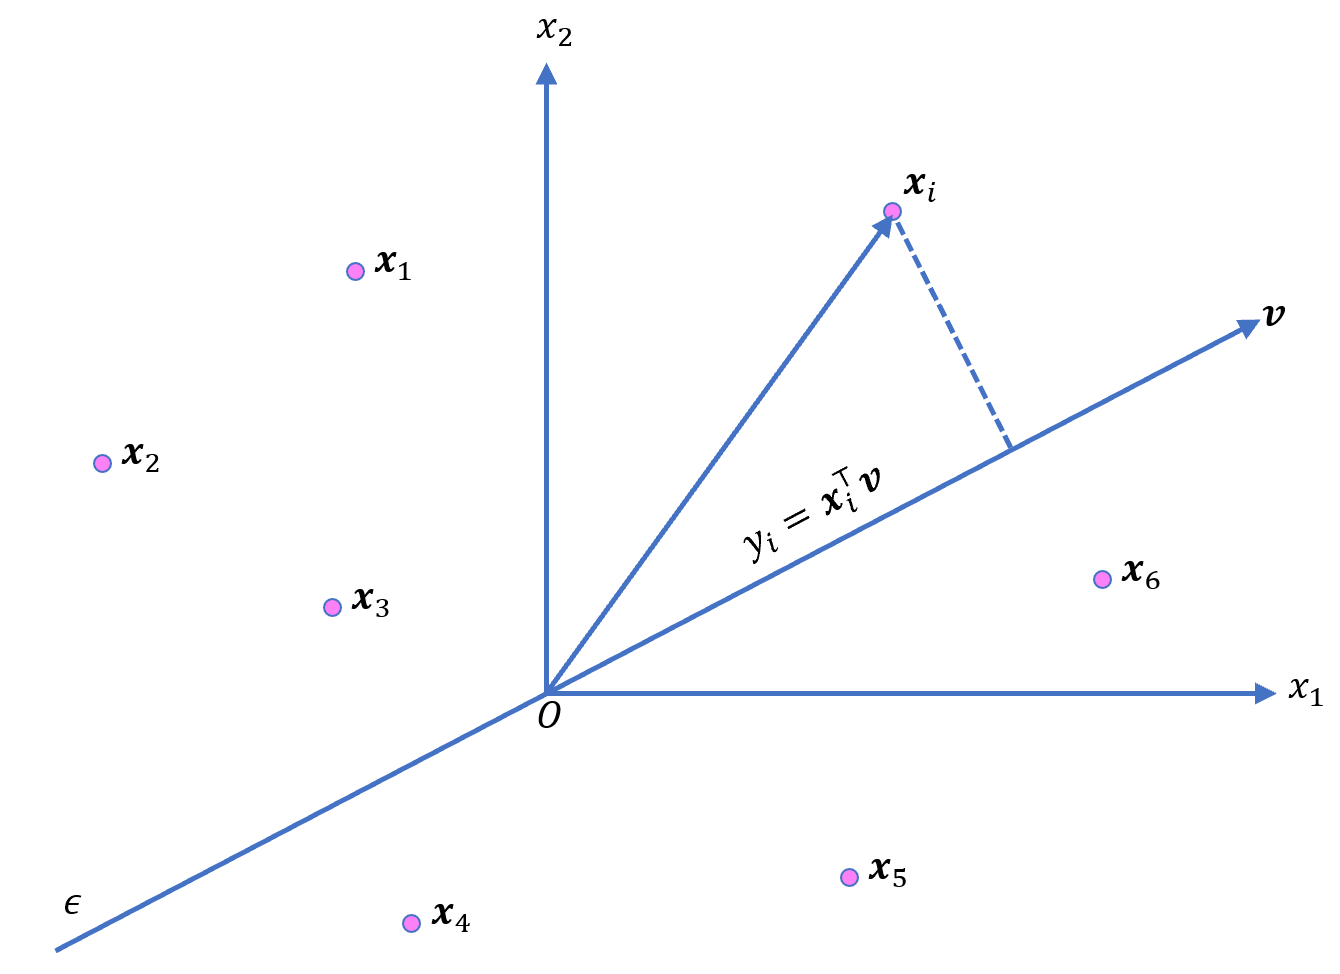
\includegraphics[width=\linewidth]{img/pca_variance_intro.png}
                \caption{Project a vector onto a direction}
            \end{figure}
        \end{column}
    \end{columns}
\end{frame}

\begin{frame}{Problem statement}
    \begin{itemize}
        \item Given $X = (\vec{X_1}, \vec{X_2},\dots,\vec{X_n}) \in \R^{m\times n}$: Data matrix
        \item $\vec{w}$ is a unit vector

        \begin{alertblock}{PCA problem}
            \begin{align*}
                &\max_{\vec{w}}\left\{\sigma^2_{P}\right\}\\
                s.t.\text{ }& \|\vec{w}\|_2 = 1
            \end{align*}
        \end{alertblock}
    \end{itemize}
\end{frame}

\subsection{Find principal components}

\begin{frame}{Find $\vec{w}$ such that $\vec{P} = X\vec{w}$, $\|\vec{w}\|_2=1$ and $\sigma^2_{P}$ is maximum}
    \begin{itemize}
        \item Consider $\sigma^2_{P}$:
    \end{itemize}
    \begin{align*}
        \sigma^2_{P} &= \E\left[ \left(\vec{x_i}^T\vec{w} - \mu_P\right)^2 \right] \quad\quad (\mu_P = \E[\vec{x_i}^T \vec{w}] = \vec{\mu_X}^T\vec{w})\\
        &= \E \left[ (X\vec{w} - \bar{X}\vec{w})^T(X\vec{w} - \bar{X}\vec{w}) \right] \\
        &= \E \left[ \vec{w}^T(X - \bar{X})^T(X - \bar{X})\vec{w} \right] \\
        &= \alert{\vec{w}^T \Sigma[X] \vec{w}} \\
        % &= \frac{1}{m} \sum_{i=1}^m{\left(\vec{w}^T\vec{x_i} - \vec{w}^T\vec{\mu_X}\right)^T \left(\vec{w}^T\vec{x_i} - \vec{w}^T\vec{\mu_X}\right)}\\
        % &= \frac{1}{m} \sum_{i=1}^m{\vec{w}^T\left(\vec{x_i} - \vec{\mu_X}\right) \left(\vec{x_i} - \vec{\mu_X}\right)^T \vec{w}} = \alert{\vec{w}^T \Sigma[X] \vec{w}}\\
        % (\Sigma[X] &= \frac{1}{m} \sum_{i=1}^m{\left(\vec{x_i} - \vec{\mu_X}\right) \left(\vec{x_i} - \vec{\mu_X}\right)^T} \text{: \textbf{Covariance matrix}})
        (\Sigma[X] &= \frac{1}{m-1}(X - \bar{X})^T(X - \bar{X}) \text{: \textbf{Unbiased covariance matrix}})
    \end{align*}
    % unbiased covariance sẽ xấp xỉ real covariance matrix hơn là bias variance
\end{frame}

\begin{frame}{Find $\vec{w}$ such that $\vec{P} = X\vec{w}$, $\|\vec{w}\|_2=1$ and $\sigma^2_{P}$ is maximum}
    \begin{itemize}
        \item Combine with constrain $\|w\|_2=1$ via \textbf{Lagrange multiplier}:
        \begin{align*}
                &\max_{\vec{w}}\left\{\vec{w}^T \Sigma[X] \vec{w} - \lambda(\vec{w}^T\vec{w} - 1)\right\}\\
                = &\max_{\vec{w}} J
            \end{align*}

        \item Solve the above problem by considering $\frac{dJ}{d\vec{w}}=0$
        \begin{align*}
            \frac{dJ}{d\vec{w}} &= \frac{d}{d\vec{w}} \left\{ \vec{w}^T \Sigma[X] \vec{w} - \lambda(\vec{w}^T\vec{w} - 1) \right\}\\
            &= I\Sigma[X] \vec{w} + \Sigma[X]^T \vec{w} - 2\lambda\vec{w}\\
            &= 2\Sigma[X]\vec{w} - 2\lambda\vec{w} = 0 \quad (\text{since } \Sigma[X] = \Sigma[X]^T)\\
            \Leftrightarrow \Sigma[X]\vec{w} &= \lambda\vec{w} \quad \text{this is \alert{Eigenvalue problem for Covariance matrix}}\\
            &\quad\quad\quad \text{in which, $\lambda$ is variance of projected data (on direction $\vec{w}$)}
        \end{align*}
    \end{itemize}
\end{frame}

\begin{frame}{Find $\vec{w}$ such that $\vec{P} = X\vec{w}$, $\|\vec{w}\|_2=1$ and $\sigma^2_{P}$ is maximum}
    \begin{columns}
        \begin{column}{0.6\textwidth}
            \begin{itemize}
                \item By solving $\Sigma[X]\vec{w} = \lambda\vec{w}$ with constrain $\|\vec{w}\|_2=1$, we obtain $n$ pairs ($n$ axes) $(\lambda, \vec{w})$ (since $\Sigma[X]\in \R^{n\times n}$)
                \item The eigenvector corresponding to the largest eigenvalue is the new axis that preserves the most information, and so on...
                \item Project data onto $\vec{w_1}$, we obtain the \textbf{first principal component}
                % \begin{align*}
                %     \alert{\vec{P_1} = \tilde{X}\vec{w_1}} \quad \text{this is the \textbf{first principal component}}
                % \end{align*}
            \end{itemize}
        \end{column}

        \begin{column}{0.4\textwidth}
            \begin{figure}
                \centering
                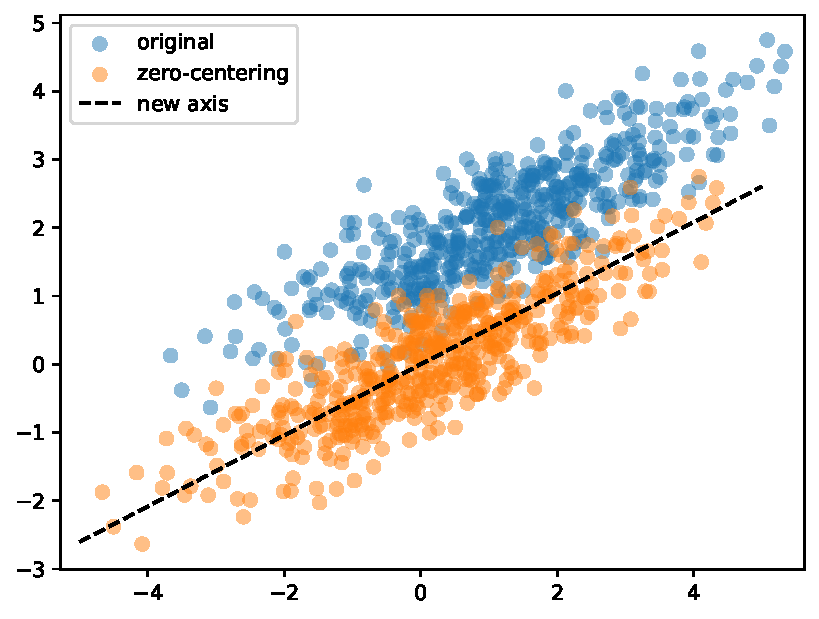
\includegraphics[width=\linewidth]{img/dp2.pdf}
                \caption{Which data to project, $X$ or $(X-\bar{X})$?}
            \end{figure}
        \end{column}
    \end{columns}
\end{frame}

\begin{frame}{PCA - Step by step}
    \begin{enumerate}
        \item Compute unbiased covariance matrix of zero-centering data: $\tilde{X} = X - \bar{X}$ % unbiased covariance sẽ xấp xỉ real covariance matrix hơn là bias variance
        $$\Sigma[X] = \frac{1}{m-1}\tilde{X}^T\tilde{X}$$

        \item Solve the eigenvalue problem to obtain $n$ pairs $(\lambda, \vec{w})$, which are $n$ directions of our data
        $$\Sigma[X]\vec{w} = \lambda \vec{w}$$

        \item Sort eigenvalues in descending order and select $k$ eigenvectors corresponding to $k$ largest eigenvalues to form $W$. \alert{Our new dataset is $P = \tilde{X}W \in \R^{m\times k}$}
        $$P = \tilde{X}W = \tilde{X} \begin{bmatrix}
            \vert     &\vert     & & \vert     \\
            \vec{w_1} &\vec{w_2} & \dots & \vec{w_k} \\
            \vert     &\vert     & & \vert     
        \end{bmatrix} = \begin{bmatrix}
            \vert     &\vert     & & \vert     \\
            \tilde{X}\vec{w_1} &\tilde{X}\vec{w_2} & \dots & \tilde{X}\vec{w_k} \\
            \vert     &\vert     & & \vert     
        \end{bmatrix}$$
    \end{enumerate}
\end{frame}

\subsection{Example}

\begin{frame}{PCA on a tabular dataset}
    \begin{columns}
        \begin{column}{0.7\textwidth}
            \begin{itemize}
                \item \uline{Problem}: Given a 2D dataset (denote $X\in \R^{3\times 2}$). Obtain the first and second component of $X$
            \end{itemize}
        \end{column}

        \begin{column}{0.4\textwidth}
            \begin{table}
                \centering
                \caption{Dataset X}
                \begin{tblr}{
                    cells = {c},
                    vline{2} = {-}{},
                    hline{1-2} = {-}{},
                }
                                 & Feature 1   & Feature 2 \\
                $\vec{x_1}^T$    & $2$         & $1$    \\
                $\vec{x_2}^T$    & $1$         & $2$    \\
                $\vec{x_3}^T$    & $0$         & $0$    
                \end{tblr}
            \end{table}
        \end{column}
    \end{columns}
\end{frame}

\begin{frame}{PCA on a tabular dataset}
    \begin{columns}
        \begin{column}{0.7\textwidth}
            \begin{itemize}
                \item \uline{Problem}: Given a 2D dataset (denote $X\in \R^{3\times 2}$). Obtain the first and second component of $X$
                \item \uline{Step 1}: Compute \textbf{unbiased covariance matrix}
                \begin{align*}
                    \tilde{X} &= X - \bar{X} = \begin{bmatrix}
                        1  & 0 \\
                        0  & 1 \\
                        -1 & -1
                    \end{bmatrix}\\
                    \Sigma[X] &= \frac{1}{2} \tilde{X}^T\tilde{X}\\
                    &= \begin{bmatrix}
                        1 & 0.5\\
                        0.5 & 1
                    \end{bmatrix}
                \end{align*}
            \end{itemize}
        \end{column}

        \begin{column}{0.4\textwidth}
            \begin{table}
                \centering
                \caption{Dataset X with means}
                \begin{tblr}{
                    cells = {c},
                    vline{2} = {-}{},
                    hline{1-2,5} = {-}{},
                }
                                 & Feature 1   & Feature 2 \\
                $\vec{x_1}^T$    & $2$         & $1$    \\
                $\vec{x_2}^T$    & $1$         & $2$    \\
                $\vec{x_3}^T$    & $0$         & $0$    \\
                                 & $\mu_1 = 1$ & $\mu_2 = 1$
                \end{tblr}
            \end{table}
        \end{column}
    \end{columns}
\end{frame}

% \begin{frame}{PCA on a tabular dataset}
%     \begin{columns}
%         \begin{column}{0.7\textwidth}
%             \begin{itemize}
%                 \item \uline{Problem}: Given a 2D dataset (denote $X\in \R^{3\times 2}$). Obtain the first and second component of $X$
%                 \item \uline{Step 2}: \textbf{Compute covariance matrix} and find its eigenvalues, eigenvectors
%                 \begin{align*}
%                     \Sigma[X] &= \frac{1}{2}X^TX\\
%                     &= \frac{1}{2}\begin{bmatrix}
%                         1 & 0 & -1\\
%                         0 & 1 & -1
%                     \end{bmatrix} \begin{bmatrix}
%                         1 & 0\\
%                         0 & 1\\
%                         -1 & -1
%                     \end{bmatrix}\\
%                     &= \begin{bmatrix}
%                         1 & 0.5\\
%                         0.5 & 1
%                     \end{bmatrix}
%                 \end{align*}
%             \end{itemize}
%         \end{column}

%         \begin{column}{0.4\textwidth}
%             \begin{table}
%                 \centering
%                 \caption{Dataset X (zero-centered)}
%                 \begin{tblr}{
%                     cells = {c},
%                     vline{2} = {-}{},
%                     hline{1-2} = {-}{},
%                 }
%                                  & Feature 1   & Feature 2 \\
%                 $\vec{x_1}^T$    & $1$         & $0$    \\
%                 $\vec{x_2}^T$    & $0$         & $1$    \\
%                 $\vec{x_3}^T$    & $-1$         & $-1$    
%                 \end{tblr}
%             \end{table}
%         \end{column}
%     \end{columns}
% \end{frame}

\begin{frame}{PCA on a tabular dataset}
    \begin{columns}
        \begin{column}{0.7\textwidth}
            \begin{itemize}
                \item \uline{Problem}: Given a 2D dataset (denote $X\in \R^{3\times 2}$). Obtain the first and second component of $X$
                \item \uline{Step 2}: Compute \textbf{eigenvalues, eigenvectors}
                \begin{align*}
                    &\Sigma[X]\vec{w} = \lambda \vec{w}\\
                    \Leftrightarrow \quad&(\Sigma[X] - \lambda I)\vec{w} = 0
                \end{align*}

                - Since $\vec{w} \neq 0 \Rightarrow \det(\Sigma[X] - \lambda I) = 0$
                \begin{align*}
                    &\det\left( \begin{bmatrix}
                        1 & 0.5\\
                        0.5 & 1
                    \end{bmatrix} - \lambda \begin{bmatrix}
                            1 & 0\\
                            0 & 1
                        \end{bmatrix} \right) = 0\\
                    \Leftrightarrow \quad &  \lambda_1 = 1.5 \text{ or } \lambda_2 = 0.5
                \end{align*}
            \end{itemize}
        \end{column}

        \begin{column}{0.3\textwidth}
            - Substitute $\lambda$ into $\Sigma[X]\vec{w} = \lambda\vec{w}$ to obtain \textbf{eigenvectors}
            \begin{align*}
                &\lambda_1 = 1.5 \rightarrow \vec{w_1} = [t, t]^T \quad (t\in \R)\\
                &\lambda_2 = 0.5 \rightarrow \vec{w_2} = [t, -t]^T \quad (t\in \R)\\
            \end{align*}

            - Since $\|w\|_2 = 1$, we obtain the normalized $\vec{w}$
            \begin{align*}
                &\vec{w_1} = \left[\frac{1}{\sqrt{2}}, \frac{1}{\sqrt{2}}\right]^T\\
                &\vec{w_2} = \left[\frac{1}{\sqrt{2}}, -\frac{1}{\sqrt{2}}\right]^T
            \end{align*}

        \end{column}
    \end{columns}
\end{frame}

\begin{frame}{PCA on a tabular dataset}
    \begin{columns}
        \begin{column}{0.6\textwidth}
            \begin{itemize}
                \item \uline{Problem}: Given a 2D dataset (denote $X\in \R^{3\times 2}$). Obtain the first and second component of $X$
                \item \uline{Step 3}: Form $W$ and compute new dataset
                \begin{align*}
                    P &= \tilde{X}W = \begin{bmatrix}
                        \vert      &\vert      \\
                        \tilde{X}\vec{w_1} &\tilde{X}\vec{w_2} \\
                        \vert      &\vert     
                    \end{bmatrix}\\
                    &= \begin{bmatrix}
                        \frac{1}{\sqrt{2}} & \frac{1}{\sqrt{2}}      \\
                        \frac{1}{\sqrt{2}} & -\frac{1}{\sqrt{2}} \\
                        -\sqrt{2}          & 0
                    \end{bmatrix}
                \end{align*}
            \end{itemize}
        \end{column}

        \begin{column}{0.4\textwidth}
            \begin{table}
                \centering
                \caption{New dataset}
                \begin{tblr}{
                    cells = {c},
                    vline{2} = {-}{},
                    hline{1-2} = {-}{},
                }
                                 & $1^{st}$ comp.   & $2^{nd}$ comp. \\
                $\vec{x_1}^T$    & $\frac{1}{\sqrt{2}} $         & $\frac{1}{\sqrt{2}}  $    \\
                $\vec{x_2}^T$    & $\frac{1}{\sqrt{2}} $         & $-\frac{1}{\sqrt{2}} $    \\
                $\vec{x_3}^T$    & $-\sqrt{2}$                   & $0$    
                \end{tblr}
            \end{table}

            \alert{How much information does $1^{st}$ comp. preserve?}
            $$R_1 = \frac{\lambda_1}{\lambda_1 + \lambda_2} = 75\%$$
        \end{column}
    \end{columns}
\end{frame}

\begin{frame}{PCA on image}
    \begin{columns}
        \begin{column}{0.6\textwidth}
            \begin{itemize}
                \item \uline{Problem}: Given a 2D image, size $(512\times 512)$. Compress the image and compare to the original one
                \item \uline{Solution}:
                \begin{itemize}
                    \item Divide the image into patches, size $(16\times 16) \rightarrow 1024$ patches
                    \item In each patch, every pixel is a feature $\rightarrow 256$ features
                    \item Obtain a tabular data of size $(1024\times 256) \to$ Perform PCA
                \end{itemize}
            \end{itemize}
        \end{column}

        \begin{column}{0.4\textwidth}
            \begin{figure}
                \centering
                
\includegraphics[width=\linewidth]{img/lena.png}
                \caption{Lena}
            \end{figure}
        \end{column}
    \end{columns}
\end{frame}

\begin{frame}{PCA on image}
    \begin{itemize}
        \item Reconstruct image from $P: \alert{\hat{X} = PW^T = \tilde{X}WW^T}$
        \item The quality of reconstructive images are lower than the original one
    \end{itemize}
    \begin{figure}
        \centering
        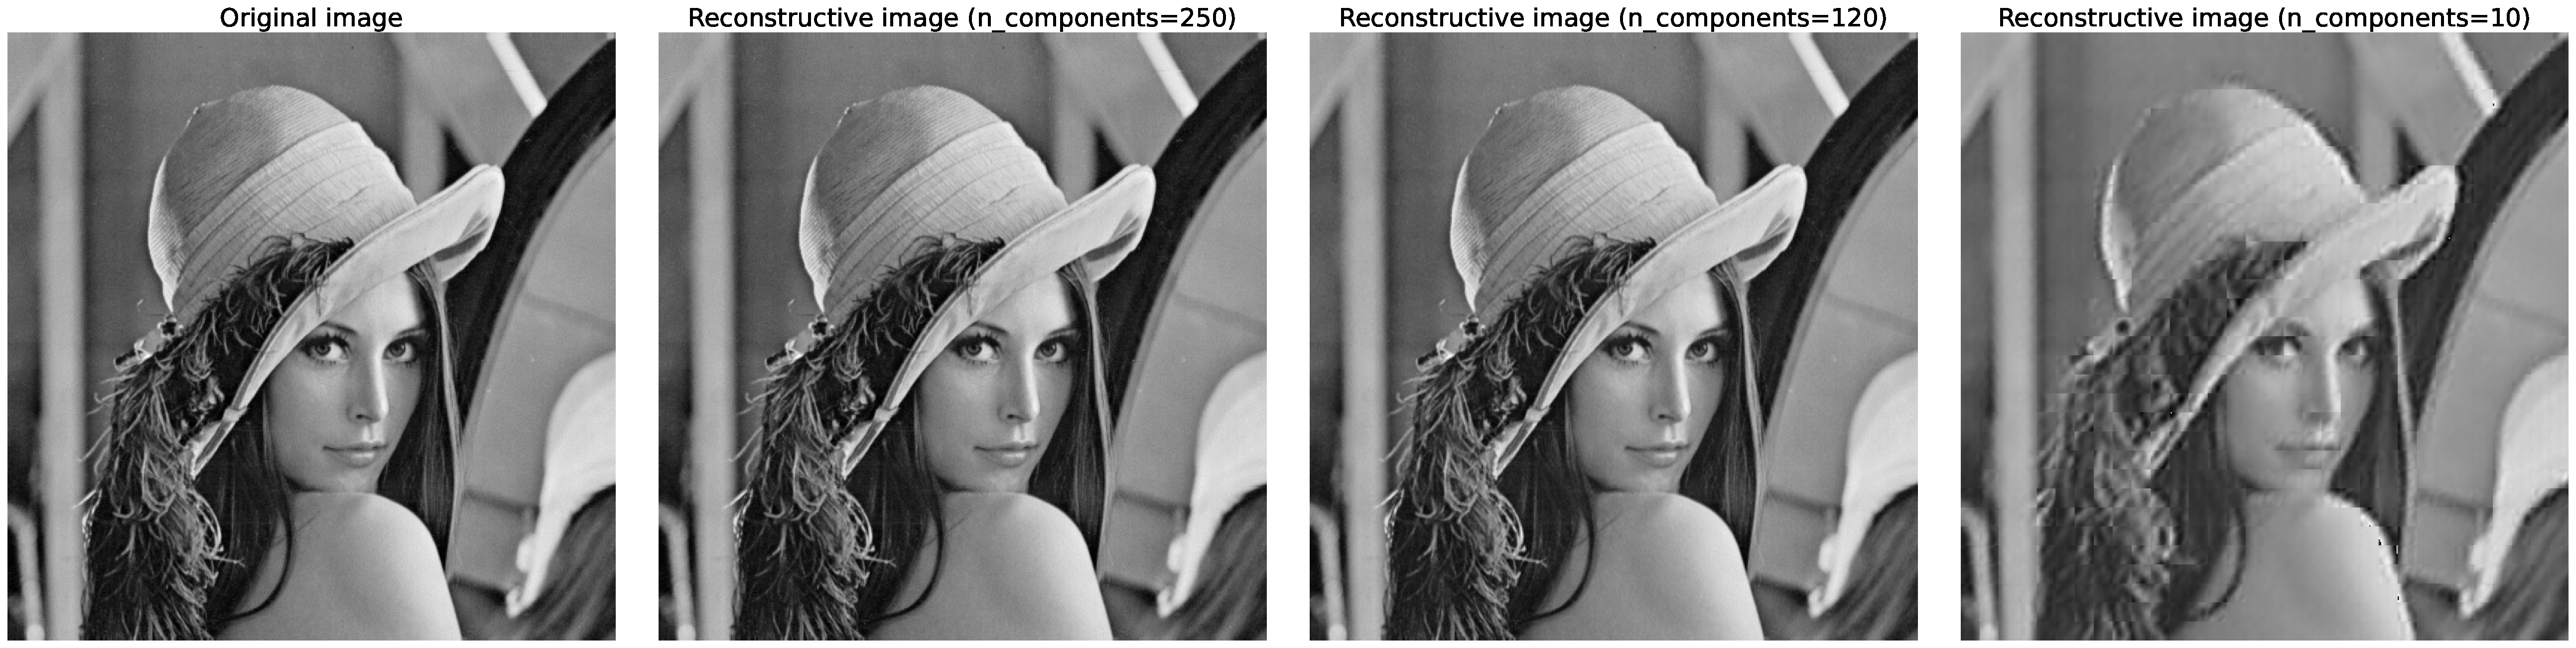
\includegraphics[width=\linewidth]{img/lena_compress1.pdf}
        \caption{Original image vs. Reconstructive images}
    \end{figure}
\end{frame}

\begin{frame}{PCA on image}
    \begin{columns}
        \begin{column}{0.5\textwidth}
            \begin{itemize}
                \item Measure the loss between original one and reconstructive ones by the distance between them
                $$L(X, \hat{X}) = d(X, \hat{X})$$
                \item In this case, we choose $l_2-norm$
                $$L(X, \hat{X}) = \|X-\hat{X}\|_2$$
            \end{itemize}
        \end{column}

        \begin{column}{0.5\textwidth}
            \begin{figure}
                \centering
                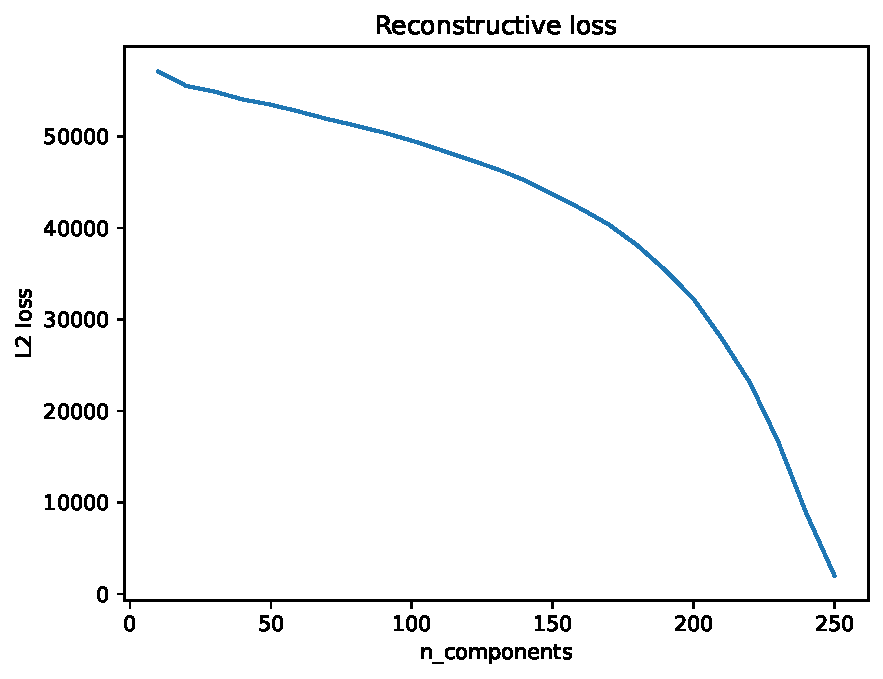
\includegraphics[width=\linewidth]{img/lena_compress_loss.pdf}
                \caption{Reconstructive loss of PCA}
            \end{figure}
        \end{column}
    \end{columns}
\end{frame}
